\documentclass[12pt letterpaper]{article}

\usepackage{fullpage}
\usepackage{graphicx}
\usepackage{amsmath}

\providecommand{\e}[1]{\ensuremath{\times 10^{#1}}}




\title{Quantum Dot Experiment}
\author{Johnny Minor \\ Partner: Kayla Mitchell}
\date{\today}

\begin{document}

\maketitle

%abstract should have a very brief overiew of the goals and main results of the experiment. 
\begin{abstract}
In this experiment we excite a semiconductor with a violet laser. Using a hand held spectrometer we determine the wavelength of light. With that we calculate the energy and then the radius of the quantum dot. Our results correspond to the expected value of 10 to 50 times the radius of an atom. 

\end{abstract}

\newpage

\section*{Description of Experiment}

The foundation of quantum mechanics is in the Schr\"{o}dinger equation. The time independent version of this equation is 
\begin{equation}
\label{schrodinger}
-\frac{\hbar^2}{2m}\frac{d^2}{dx^2} \psi + V(x) \psi = E \psi
\end{equation}

where $m$ is the mass of the particle, $V(x)$ is the potential, $E$ are the energy levels, and $\psi$ is the wave function for which we want to solve for. When we set the potential function to be 

$$
V(x) = 
\begin{cases} 
      0 & 0 < x < L  \\
      \infty & x \leq 0 \\
      \infty & x \geq 0 \\
   \end{cases}
$$

where $L$ is the length of the region or box. This is the familiar infinite square well potential. We know the form of the solution to a second order differential equation like equation \ref{schrodinger} quite well. They will be period functions. However, we must apply the appropriate boundary conditions to find our particular solution for this problem with the specific potential function $V(x)$. Once the the boundary conditions have been applied we have our solution 
$$ 
\psi(x) = \sqrt{\frac{2}{L}} \sin(\frac{n \pi}{L} \cdot x)
$$
$$ 
E = \frac{n^2 \hbar^2 \pi^2 }{2mL^2} \quad \mathrm{where} \quad n = 1, 2, 3, \dots
$$

However, this is for an infinite square well. Which our experiment was not. So we needed to make corrections and instead say $L = R$. Where $R$ is the radius of the quantum dot that we were trying to measure. 

In our experiment we shined a laser at the quantum dot which would then excite the electron across the band gap into the conductance band. This would also create a hole in the valence band. Once the electron went back down to the valence band it would emit a photon. The total energy of that photon emitted will be a sum of the energies from the hole, the electron, and the band gap. We can express this as 
\begin{equation}
\label{gamma_energy}
E_{\gamma} = \frac{\pi^2 \hbar^2}{2 m_e^* R^2} + \frac{\pi^2 \hbar^2}{2 m_h^* R^2} + E_{\mathrm{gap}}
\end{equation}
where $m_e^*$ is the mass of the electron, $m_h^*$ is the mass of the hole, and $E_{\mathrm{gap}}$ is the energy of the band gap. Since we know the relationship
\begin{equation}
\label{energy} 
E = hf = \frac{h c}{\lambda}
\end{equation}
Then we set them equal and measure the wavelength to get the energy. Once we have the energy we can then rearrange our equation to solve for $R$. We will then know the radius of our quantum dot. 

$$
\frac{h c}{\lambda} = \frac{\pi^2 \hbar^2}{2 m_e^* R^2} + \frac{\pi^2 \hbar^2}{2 m_h^* R^2} + E_{\mathrm{gap}}
$$

if set $ hc / \lambda = A $ and solve for $R$ then we end up with 
\begin{equation}
\label{radius}
R = \left( \frac{\pi^2 \hbar^2}{2(A-E_{gap}) m_e^*} + \frac{\pi^2 \hbar^2}{2(A-E_{gap}) m_h^*} \right)^{1/2}
\end{equation}

So the aim in experiment is that while one partner shines a violet laser at each sample the other will look through the spectrometer. We use a violet laser because the red laser will not excite the electron into the conduction band. They will attempt to read where the line of emission shows up as accurately as the spectrometer will allow. This value will be recorded and compared then using the best fit line for the ceiling lights to get a corrected wavelength. This wavelength can then be put in to find the radius of the quantum dot. 


\section*{Data and Analysis}

We first found the spectrum of the fluorescent bulbs in the room. We then comapred the values we found with those online. We created a scatter plot and ran a linear regression fit. When there was a range of values the average was taken. 
\begin{center}
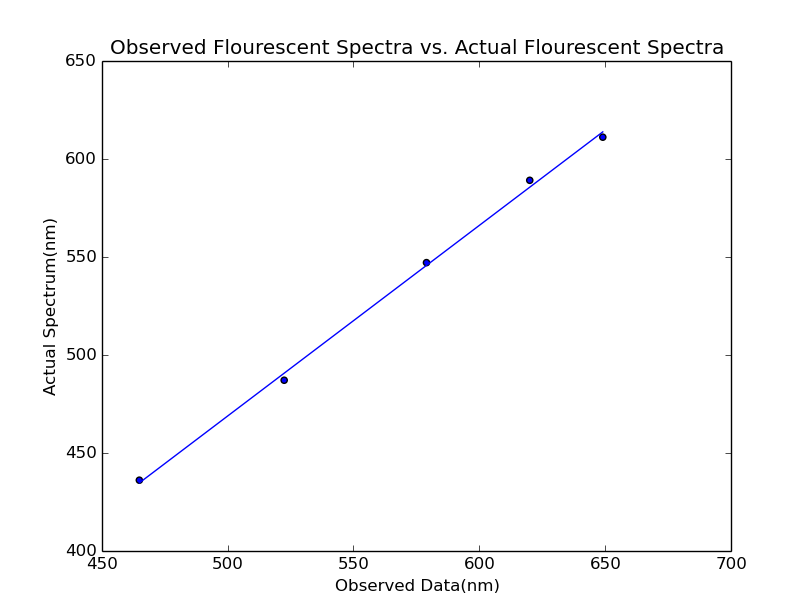
\includegraphics[width=0.75\textwidth]{spectra.png}
\end{center}

\noindent The equation of the best fit line was $y = 0.9733 x - 17.97$. This equation enables us to translate our observed values into actual values. 

%In the first vial we noted the sample turned a green color when the violet laser was applied. We noted a band in the spectrometer from 540 nm to 590 nm. If we apply the best fit equation then we find the actual wavelength range to be from 507.61 -- 556.23 nm. If we use equation \ref{energy} then we find the energy to be %TODO: calculate this value!  . 
%We can then use those values of energy to find the radius of the quantum dot using equation \ref{radius}. The values we found for the radius of the first sample was %TODO: add this value. 

The range of values read off from all five samples was recorded. We then used equation \ref{energy} to calculate the energy. With that value we were able to then able to calculate that samples quantum dot radius. The values can be easily read off from a table. 

\begin{table}[ht!] %difference between a table and a figure? Nothing other than the name. 
\caption{Summary of results from quantum dot}
\label{tab:results}
\begin{tabular}{| p{1.25cm} | p{2.25cm} | p{1.5cm} | p{1.5cm} | p{2.25cm} | p{2.25cm}|}
\hline
Sample Number & Observed Color & Observed $\lambda$ (nm) & Calculated $\lambda$ (nm) & Energy(J) &  Calculated Radius(m) \\ 
\hline
1 & green & 540 -- 590 & 507.61 -- 556.23  & 3.91\e{-19} -- 3.57\e{-19}  & 2.19\e{-9} -- 2.44\e{-9}  \\
\hline
2 & green/red & 550 -- 630 & 517.35 -- 595.21  & 3.84\e{-19} -- 3.34\e{-19}   & 2.24\e{-9} -- 2.67\e{-9}   \\
\hline
3 & orange  & 590 -- 660 & 556.277 -- 624.41 & 3.57\e{-19} -- 3.18\e{-19}  & 2.44\e{-9} -- 2.87\e{-9} \\
\hline
4 & reddish/orange & 630 -- 670 & 595.21 -- 634.141  & 3.34\e{-19} -- 3.13\e{-19} & 2.67\e{-9} -- 2.94\e{-9} \\ 
\hline
\end{tabular}
\end{table}
\section*{Results and Conclusions}

From the experiment manual we would expect to find a diameter of the quantum dot in the range of 10-50 times that of an atom. The diameter of an atom is on the order of 1\e{-10} m.
So, our findings are seemingly accurate. 

From equation \ref{gamma_energy} we can take the limit as R goes to infinity and see that the energy becomes $E_{gap}$. This is important to notice because this would mean that the radius would be very large and the equation would essentially have no curvature, and therefore have zero energy. 

\bigskip

\noindent \textbf{Additional Questions:}

\begin{itemize}
\item We use the violet laser because the red laser does not have enough energy to excite the electron into the conduction band. This meant that it would then not emit a photon. Which means that we wouldn't be able to use the spectrometer. 

\item A spectrometer works by reflecting the incoming light onto a grading. The grading will then separate the frequencies. It will then bounce them off another mirror. Finally the frequencies will be projected onto a surface where they can be read off. 

\item The overhead light is a fluorescent bulb which has many different elements inside it that emit light. Each element has a peak that we were able to record. The overhead projector spectra looks like a rainbow because it gets scattered like a light going through a prism emits the full rainbow of colors. 
\end{itemize}



\end{document}